\documentclass[a4paper,12pt]{article}
\usepackage[margin=18mm]{geometry}
\usepackage{tikz}
\usepackage{amsmath}
\newcommand{\pFourCell}[2]{\makebox[#1em][c]{\ensuremath{#2}}}
\pagestyle{empty}
\begin{document}
\section*{Spaltentreue LaTeX-Ausgabe}
\noindent Gleichung: \texttt{sin(sqrt((x+3)/(2+1)))=5} \hfill Zielvariable: \texttt{x} \hfill Profil: \texttt{standard}

\vspace{8mm}
\begin{center}
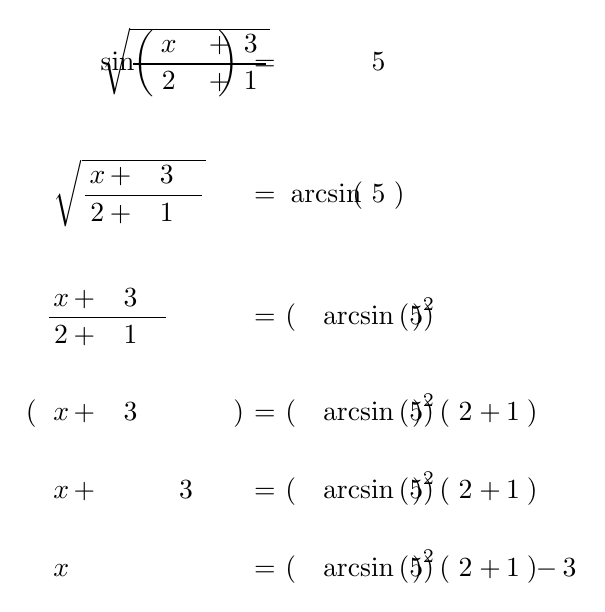
\begin{tikzpicture}[x=1em,y=-1em]
\node[anchor=base, inner sep=0pt] at (5.72,2.9) {$\pFourCell{4.8}{\sqrt{\displaystyle\frac{\pFourCell{2.56}{x}\pFourCell{1.12}{+}\pFourCell{1.12}{3}}{\pFourCell{2.56}{2}\pFourCell{1.12}{+}\pFourCell{1.12}{1}}}}$};
\node[anchor=base, inner sep=0pt] at (3.25,2.9) {$\pFourCell{1.62}{\sin}$};
\node[anchor=base, inner sep=0pt] at (4.25,2.9) {$\pFourCell{0.38}{\left(\vphantom{\pFourCell{4.8}{\sqrt{\displaystyle\frac{\pFourCell{2.56}{x}\pFourCell{1.12}{+}\pFourCell{1.12}{3}}{\pFourCell{2.56}{2}\pFourCell{1.12}{+}\pFourCell{1.12}{1}}}}}\right.}$};
\node[anchor=base, inner sep=0pt] at (7.19,2.9) {$\pFourCell{0.38}{\left.\vphantom{\pFourCell{4.8}{\sqrt{\displaystyle\frac{\pFourCell{2.56}{x}\pFourCell{1.12}{+}\pFourCell{1.12}{3}}{\pFourCell{2.56}{2}\pFourCell{1.12}{+}\pFourCell{1.12}{1}}}}}\right)}$};
\node[anchor=base, inner sep=0pt] at (8.57,2.9) {$=$};
\node[anchor=base, inner sep=0pt] at (12.68,2.9) {$5$};
\node[anchor=base, inner sep=0pt] at (3.69,7.65) {$\pFourCell{4.62}{\sqrt{\displaystyle\frac{\pFourCell{0.9}{x}\pFourCell{0.78}{+}\pFourCell{2.56}{3}}{\pFourCell{0.9}{2}\pFourCell{0.78}{+}\pFourCell{2.56}{1}}}}$};
\node[anchor=base, inner sep=0pt] at (8.57,7.65) {$=$};
\node[anchor=base, inner sep=0pt] at (12.68,7.65) {$\pFourCell{1}{5}$};
\node[anchor=base, inner sep=0pt] at (10.78,7.65) {$\pFourCell{2.04}{\arcsin}$};
\node[anchor=base, inner sep=0pt] at (11.99,7.65) {$\pFourCell{0.38}{\left(\vphantom{\pFourCell{1}{5}}\right.}$};
\node[anchor=base, inner sep=0pt] at (13.37,7.65) {$\pFourCell{0.38}{\left.\vphantom{\pFourCell{1}{5}}\right)}$};
\node[anchor=base, inner sep=0pt] at (2.88,12.075) {$\displaystyle\frac{\pFourCell{0.9}{x}\pFourCell{0.78}{+}\pFourCell{2.56}{3}}{\pFourCell{0.9}{2}\pFourCell{0.78}{+}\pFourCell{2.56}{1}}$};
\node[anchor=base, inner sep=0pt] at (8.57,12.075) {$=$};
\node[anchor=base, inner sep=0pt] at (12.68,12.075) {$\pFourCell{1}{\arcsin\left(5\right)}$};
\node[anchor=base, inner sep=0pt] at (9.57,12.075) {$\pFourCell{0.38}{\left(\vphantom{\pFourCell{1}{\arcsin\left(5\right)}}\right.}$};
\node[anchor=base, inner sep=0pt] at (14.25,12.075) {$\pFourCell{1.38}{\left.\vphantom{\pFourCell{1}{\arcsin\left(5\right)}}\right)^{2}}$};
\node[anchor=base, inner sep=0pt] at (2.88,15.535) {$\pFourCell{0.9}{x}\pFourCell{0.78}{+}\pFourCell{2.56}{3}$};
\node[anchor=base, inner sep=0pt] at (0.19,15.535) {$\pFourCell{0.38}{\left(\vphantom{\pFourCell{0.9}{x}\pFourCell{0.78}{+}\pFourCell{2.56}{3}}\right.}$};
\node[anchor=base, inner sep=0pt] at (7.57,15.535) {$\pFourCell{0.38}{\left.\vphantom{\pFourCell{0.9}{x}\pFourCell{0.78}{+}\pFourCell{2.56}{3}}\right)}$};
\node[anchor=base, inner sep=0pt] at (8.57,15.535) {$=$};
\node[anchor=base, inner sep=0pt] at (12.68,15.535) {$\pFourCell{1}{\arcsin\left(5\right)}$};
\node[anchor=base, inner sep=0pt] at (9.57,15.535) {$\pFourCell{0.38}{\left(\vphantom{\pFourCell{1}{\arcsin\left(5\right)}}\right.}$};
\node[anchor=base, inner sep=0pt] at (14.25,15.535) {$\pFourCell{1.38}{\left.\vphantom{\pFourCell{1}{\arcsin\left(5\right)}}\right)^{2}}$};
\node[anchor=base, inner sep=0pt] at (16.65,15.535) {$\pFourCell{1}{2}\pFourCell{0.78}{+}\pFourCell{0.88}{1}$};
\node[anchor=base, inner sep=0pt] at (15.13,15.535) {$\pFourCell{0.38}{\left(\vphantom{\pFourCell{1}{2}\pFourCell{0.78}{+}\pFourCell{0.88}{1}}\right.}$};
\node[anchor=base, inner sep=0pt] at (18.17,15.535) {$\pFourCell{0.38}{\left.\vphantom{\pFourCell{1}{2}\pFourCell{0.78}{+}\pFourCell{0.88}{1}}\right)}$};
\node[anchor=base, inner sep=0pt] at (1.21,18.355) {$x$};
\node[anchor=base, inner sep=0pt] at (2.05,18.355) {$+$};
\node[anchor=base, inner sep=0pt] at (5.72,18.355) {$3$};
\node[anchor=base, inner sep=0pt] at (8.57,18.355) {$=$};
\node[anchor=base, inner sep=0pt] at (12.68,18.355) {$\pFourCell{1}{\arcsin\left(5\right)}$};
\node[anchor=base, inner sep=0pt] at (9.57,18.355) {$\pFourCell{0.38}{\left(\vphantom{\pFourCell{1}{\arcsin\left(5\right)}}\right.}$};
\node[anchor=base, inner sep=0pt] at (14.25,18.355) {$\pFourCell{1.38}{\left.\vphantom{\pFourCell{1}{\arcsin\left(5\right)}}\right)^{2}}$};
\node[anchor=base, inner sep=0pt] at (16.65,18.355) {$\pFourCell{1}{2}\pFourCell{0.78}{+}\pFourCell{0.88}{1}$};
\node[anchor=base, inner sep=0pt] at (15.13,18.355) {$\pFourCell{0.38}{\left(\vphantom{\pFourCell{1}{2}\pFourCell{0.78}{+}\pFourCell{0.88}{1}}\right.}$};
\node[anchor=base, inner sep=0pt] at (18.17,18.355) {$\pFourCell{0.38}{\left.\vphantom{\pFourCell{1}{2}\pFourCell{0.78}{+}\pFourCell{0.88}{1}}\right)}$};
\node[anchor=base, inner sep=0pt] at (1.21,21.175) {$x$};
\node[anchor=base, inner sep=0pt] at (8.57,21.175) {$=$};
\node[anchor=base, inner sep=0pt] at (12.68,21.175) {$\pFourCell{1}{\arcsin\left(5\right)}$};
\node[anchor=base, inner sep=0pt] at (9.57,21.175) {$\pFourCell{0.38}{\left(\vphantom{\pFourCell{1}{\arcsin\left(5\right)}}\right.}$};
\node[anchor=base, inner sep=0pt] at (14.25,21.175) {$\pFourCell{1.38}{\left.\vphantom{\pFourCell{1}{\arcsin\left(5\right)}}\right)^{2}}$};
\node[anchor=base, inner sep=0pt] at (16.65,21.175) {$\pFourCell{1}{2}\pFourCell{0.78}{+}\pFourCell{0.88}{1}$};
\node[anchor=base, inner sep=0pt] at (15.13,21.175) {$\pFourCell{0.38}{\left(\vphantom{\pFourCell{1}{2}\pFourCell{0.78}{+}\pFourCell{0.88}{1}}\right.}$};
\node[anchor=base, inner sep=0pt] at (18.17,21.175) {$\pFourCell{0.38}{\left.\vphantom{\pFourCell{1}{2}\pFourCell{0.78}{+}\pFourCell{0.88}{1}}\right)}$};
\node[anchor=base, inner sep=0pt] at (18.75,21.175) {$-$};
\node[anchor=base, inner sep=0pt] at (19.58,21.175) {$3$};
\end{tikzpicture}
\end{center}

\newpage
\section*{Spaltentreue LaTeX-Ausgabe mit Spaltengrenzen}
\vspace{6mm}
\begin{center}
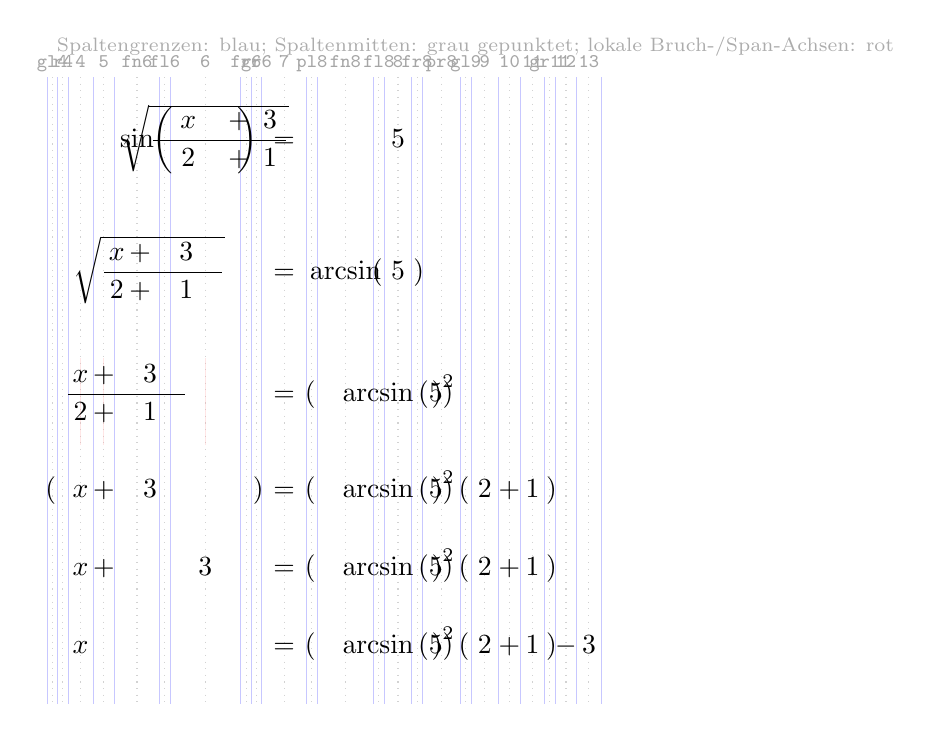
\begin{tikzpicture}[x=1em,y=-1em]
\node[font={\scriptsize}, text=gray!65, anchor=west] at (0,-0.75) {Spaltengrenzen: blau; Spaltenmitten: grau gepunktet; lokale Bruch-/Span-Achsen: rot};
\draw[blue!22, line width=0.28pt] (0,0.35) -- (0,23.01);
\draw[blue!22, line width=0.28pt] (0.38,0.35) -- (0.38,23.01);
\draw[blue!22, line width=0.28pt] (0.76,0.35) -- (0.76,23.01);
\draw[blue!22, line width=0.28pt] (1.66,0.35) -- (1.66,23.01);
\draw[blue!22, line width=0.28pt] (2.44,0.35) -- (2.44,23.01);
\draw[blue!22, line width=0.28pt] (4.06,0.35) -- (4.06,23.01);
\draw[blue!22, line width=0.28pt] (4.44,0.35) -- (4.44,23.01);
\draw[blue!22, line width=0.28pt] (7,0.35) -- (7,23.01);
\draw[blue!22, line width=0.28pt] (7.38,0.35) -- (7.38,23.01);
\draw[blue!22, line width=0.28pt] (7.76,0.35) -- (7.76,23.01);
\draw[blue!22, line width=0.28pt] (9.38,0.35) -- (9.38,23.01);
\draw[blue!22, line width=0.28pt] (9.76,0.35) -- (9.76,23.01);
\draw[blue!22, line width=0.28pt] (11.8,0.35) -- (11.8,23.01);
\draw[blue!22, line width=0.28pt] (12.18,0.35) -- (12.18,23.01);
\draw[blue!22, line width=0.28pt] (13.18,0.35) -- (13.18,23.01);
\draw[blue!22, line width=0.28pt] (13.56,0.35) -- (13.56,23.01);
\draw[blue!22, line width=0.28pt] (14.94,0.35) -- (14.94,23.01);
\draw[blue!22, line width=0.28pt] (15.32,0.35) -- (15.32,23.01);
\draw[blue!22, line width=0.28pt] (16.32,0.35) -- (16.32,23.01);
\draw[blue!22, line width=0.28pt] (17.1,0.35) -- (17.1,23.01);
\draw[blue!22, line width=0.28pt] (17.98,0.35) -- (17.98,23.01);
\draw[blue!22, line width=0.28pt] (18.36,0.35) -- (18.36,23.01);
\draw[blue!22, line width=0.28pt] (19.14,0.35) -- (19.14,23.01);
\draw[blue!22, line width=0.28pt] (20.02,0.35) -- (20.02,23.01);
\draw[gray!35, dotted] (0.19,0.35) -- (0.19,23.01);
\node[font={\ttfamily\scriptsize}, text=gray!70, anchor=base] at (0.19,0) {gl4};
\draw[gray!35, dotted] (0.57,0.35) -- (0.57,23.01);
\node[font={\ttfamily\scriptsize}, text=gray!70, anchor=base] at (0.57,0) {r4};
\draw[gray!35, dotted] (1.21,0.35) -- (1.21,23.01);
\node[font={\ttfamily\scriptsize}, text=gray!70, anchor=base] at (1.21,0) {4};
\draw[gray!35, dotted] (2.05,0.35) -- (2.05,23.01);
\node[font={\ttfamily\scriptsize}, text=gray!70, anchor=base] at (2.05,0) {5};
\draw[gray!35, dotted] (3.25,0.35) -- (3.25,23.01);
\node[font={\ttfamily\scriptsize}, text=gray!70, anchor=base] at (3.25,0) {fn6};
\draw[gray!35, dotted] (4.25,0.35) -- (4.25,23.01);
\node[font={\ttfamily\scriptsize}, text=gray!70, anchor=base] at (4.25,0) {fl6};
\draw[gray!35, dotted] (5.72,0.35) -- (5.72,23.01);
\node[font={\ttfamily\scriptsize}, text=gray!70, anchor=base] at (5.72,0) {6};
\draw[gray!35, dotted] (7.19,0.35) -- (7.19,23.01);
\node[font={\ttfamily\scriptsize}, text=gray!70, anchor=base] at (7.19,0) {fr6};
\draw[gray!35, dotted] (7.57,0.35) -- (7.57,23.01);
\node[font={\ttfamily\scriptsize}, text=gray!70, anchor=base] at (7.57,0) {gr6};
\draw[gray!35, dotted] (8.57,0.35) -- (8.57,23.01);
\node[font={\ttfamily\scriptsize}, text=gray!70, anchor=base] at (8.57,0) {7};
\draw[gray!35, dotted] (9.57,0.35) -- (9.57,23.01);
\node[font={\ttfamily\scriptsize}, text=gray!70, anchor=base] at (9.57,0) {pl8};
\draw[gray!35, dotted] (10.78,0.35) -- (10.78,23.01);
\node[font={\ttfamily\scriptsize}, text=gray!70, anchor=base] at (10.78,0) {fn8};
\draw[gray!35, dotted] (11.99,0.35) -- (11.99,23.01);
\node[font={\ttfamily\scriptsize}, text=gray!70, anchor=base] at (11.99,0) {fl8};
\draw[gray!35, dotted] (12.68,0.35) -- (12.68,23.01);
\node[font={\ttfamily\scriptsize}, text=gray!70, anchor=base] at (12.68,0) {8};
\draw[gray!35, dotted] (13.37,0.35) -- (13.37,23.01);
\node[font={\ttfamily\scriptsize}, text=gray!70, anchor=base] at (13.37,0) {fr8};
\draw[gray!35, dotted] (14.25,0.35) -- (14.25,23.01);
\node[font={\ttfamily\scriptsize}, text=gray!70, anchor=base] at (14.25,0) {pr8};
\draw[gray!35, dotted] (15.13,0.35) -- (15.13,23.01);
\node[font={\ttfamily\scriptsize}, text=gray!70, anchor=base] at (15.13,0) {gl9};
\draw[gray!35, dotted] (15.82,0.35) -- (15.82,23.01);
\node[font={\ttfamily\scriptsize}, text=gray!70, anchor=base] at (15.82,0) {9};
\draw[gray!35, dotted] (16.71,0.35) -- (16.71,23.01);
\node[font={\ttfamily\scriptsize}, text=gray!70, anchor=base] at (16.71,0) {10};
\draw[gray!35, dotted] (17.54,0.35) -- (17.54,23.01);
\node[font={\ttfamily\scriptsize}, text=gray!70, anchor=base] at (17.54,0) {11};
\draw[gray!35, dotted] (18.17,0.35) -- (18.17,23.01);
\node[font={\ttfamily\scriptsize}, text=gray!70, anchor=base] at (18.17,0) {gr11};
\draw[gray!35, dotted] (18.75,0.35) -- (18.75,23.01);
\node[font={\ttfamily\scriptsize}, text=gray!70, anchor=base] at (18.75,0) {12};
\draw[gray!35, dotted] (19.58,0.35) -- (19.58,23.01);
\node[font={\ttfamily\scriptsize}, text=gray!70, anchor=base] at (19.58,0) {13};
\node[anchor=base, inner sep=0pt] at (5.72,2.9) {$\pFourCell{4.8}{\sqrt{\displaystyle\frac{\pFourCell{2.56}{x}\pFourCell{1.12}{+}\pFourCell{1.12}{3}}{\pFourCell{2.56}{2}\pFourCell{1.12}{+}\pFourCell{1.12}{1}}}}$};
\node[anchor=base, inner sep=0pt] at (3.25,2.9) {$\pFourCell{1.62}{\sin}$};
\node[anchor=base, inner sep=0pt] at (4.25,2.9) {$\pFourCell{0.38}{\left(\vphantom{\pFourCell{4.8}{\sqrt{\displaystyle\frac{\pFourCell{2.56}{x}\pFourCell{1.12}{+}\pFourCell{1.12}{3}}{\pFourCell{2.56}{2}\pFourCell{1.12}{+}\pFourCell{1.12}{1}}}}}\right.}$};
\node[anchor=base, inner sep=0pt] at (7.19,2.9) {$\pFourCell{0.38}{\left.\vphantom{\pFourCell{4.8}{\sqrt{\displaystyle\frac{\pFourCell{2.56}{x}\pFourCell{1.12}{+}\pFourCell{1.12}{3}}{\pFourCell{2.56}{2}\pFourCell{1.12}{+}\pFourCell{1.12}{1}}}}}\right)}$};
\node[anchor=base, inner sep=0pt] at (8.57,2.9) {$=$};
\node[anchor=base, inner sep=0pt] at (12.68,2.9) {$5$};
\node[anchor=base, inner sep=0pt] at (3.69,7.65) {$\pFourCell{4.62}{\sqrt{\displaystyle\frac{\pFourCell{0.9}{x}\pFourCell{0.78}{+}\pFourCell{2.56}{3}}{\pFourCell{0.9}{2}\pFourCell{0.78}{+}\pFourCell{2.56}{1}}}}$};
\node[anchor=base, inner sep=0pt] at (8.57,7.65) {$=$};
\node[anchor=base, inner sep=0pt] at (12.68,7.65) {$\pFourCell{1}{5}$};
\node[anchor=base, inner sep=0pt] at (10.78,7.65) {$\pFourCell{2.04}{\arcsin}$};
\node[anchor=base, inner sep=0pt] at (11.99,7.65) {$\pFourCell{0.38}{\left(\vphantom{\pFourCell{1}{5}}\right.}$};
\node[anchor=base, inner sep=0pt] at (13.37,7.65) {$\pFourCell{0.38}{\left.\vphantom{\pFourCell{1}{5}}\right)}$};
\draw[red!30, opacity=0.32, line width=0.35pt] (1.21,10.5) -- (1.21,13.65);
\draw[red!30, opacity=0.32, line width=0.35pt] (2.05,10.5) -- (2.05,13.65);
\draw[red!30, opacity=0.32, line width=0.35pt] (5.72,10.5) -- (5.72,13.65);
\node[anchor=base, inner sep=0pt] at (2.88,12.075) {$\displaystyle\frac{\pFourCell{0.9}{x}\pFourCell{0.78}{+}\pFourCell{2.56}{3}}{\pFourCell{0.9}{2}\pFourCell{0.78}{+}\pFourCell{2.56}{1}}$};
\node[anchor=base, inner sep=0pt] at (8.57,12.075) {$=$};
\node[anchor=base, inner sep=0pt] at (12.68,12.075) {$\pFourCell{1}{\arcsin\left(5\right)}$};
\node[anchor=base, inner sep=0pt] at (9.57,12.075) {$\pFourCell{0.38}{\left(\vphantom{\pFourCell{1}{\arcsin\left(5\right)}}\right.}$};
\node[anchor=base, inner sep=0pt] at (14.25,12.075) {$\pFourCell{1.38}{\left.\vphantom{\pFourCell{1}{\arcsin\left(5\right)}}\right)^{2}}$};
\node[anchor=base, inner sep=0pt] at (2.88,15.535) {$\pFourCell{0.9}{x}\pFourCell{0.78}{+}\pFourCell{2.56}{3}$};
\node[anchor=base, inner sep=0pt] at (0.19,15.535) {$\pFourCell{0.38}{\left(\vphantom{\pFourCell{0.9}{x}\pFourCell{0.78}{+}\pFourCell{2.56}{3}}\right.}$};
\node[anchor=base, inner sep=0pt] at (7.57,15.535) {$\pFourCell{0.38}{\left.\vphantom{\pFourCell{0.9}{x}\pFourCell{0.78}{+}\pFourCell{2.56}{3}}\right)}$};
\node[anchor=base, inner sep=0pt] at (8.57,15.535) {$=$};
\node[anchor=base, inner sep=0pt] at (12.68,15.535) {$\pFourCell{1}{\arcsin\left(5\right)}$};
\node[anchor=base, inner sep=0pt] at (9.57,15.535) {$\pFourCell{0.38}{\left(\vphantom{\pFourCell{1}{\arcsin\left(5\right)}}\right.}$};
\node[anchor=base, inner sep=0pt] at (14.25,15.535) {$\pFourCell{1.38}{\left.\vphantom{\pFourCell{1}{\arcsin\left(5\right)}}\right)^{2}}$};
\node[anchor=base, inner sep=0pt] at (16.65,15.535) {$\pFourCell{1}{2}\pFourCell{0.78}{+}\pFourCell{0.88}{1}$};
\node[anchor=base, inner sep=0pt] at (15.13,15.535) {$\pFourCell{0.38}{\left(\vphantom{\pFourCell{1}{2}\pFourCell{0.78}{+}\pFourCell{0.88}{1}}\right.}$};
\node[anchor=base, inner sep=0pt] at (18.17,15.535) {$\pFourCell{0.38}{\left.\vphantom{\pFourCell{1}{2}\pFourCell{0.78}{+}\pFourCell{0.88}{1}}\right)}$};
\node[anchor=base, inner sep=0pt] at (1.21,18.355) {$x$};
\node[anchor=base, inner sep=0pt] at (2.05,18.355) {$+$};
\node[anchor=base, inner sep=0pt] at (5.72,18.355) {$3$};
\node[anchor=base, inner sep=0pt] at (8.57,18.355) {$=$};
\node[anchor=base, inner sep=0pt] at (12.68,18.355) {$\pFourCell{1}{\arcsin\left(5\right)}$};
\node[anchor=base, inner sep=0pt] at (9.57,18.355) {$\pFourCell{0.38}{\left(\vphantom{\pFourCell{1}{\arcsin\left(5\right)}}\right.}$};
\node[anchor=base, inner sep=0pt] at (14.25,18.355) {$\pFourCell{1.38}{\left.\vphantom{\pFourCell{1}{\arcsin\left(5\right)}}\right)^{2}}$};
\node[anchor=base, inner sep=0pt] at (16.65,18.355) {$\pFourCell{1}{2}\pFourCell{0.78}{+}\pFourCell{0.88}{1}$};
\node[anchor=base, inner sep=0pt] at (15.13,18.355) {$\pFourCell{0.38}{\left(\vphantom{\pFourCell{1}{2}\pFourCell{0.78}{+}\pFourCell{0.88}{1}}\right.}$};
\node[anchor=base, inner sep=0pt] at (18.17,18.355) {$\pFourCell{0.38}{\left.\vphantom{\pFourCell{1}{2}\pFourCell{0.78}{+}\pFourCell{0.88}{1}}\right)}$};
\node[anchor=base, inner sep=0pt] at (1.21,21.175) {$x$};
\node[anchor=base, inner sep=0pt] at (8.57,21.175) {$=$};
\node[anchor=base, inner sep=0pt] at (12.68,21.175) {$\pFourCell{1}{\arcsin\left(5\right)}$};
\node[anchor=base, inner sep=0pt] at (9.57,21.175) {$\pFourCell{0.38}{\left(\vphantom{\pFourCell{1}{\arcsin\left(5\right)}}\right.}$};
\node[anchor=base, inner sep=0pt] at (14.25,21.175) {$\pFourCell{1.38}{\left.\vphantom{\pFourCell{1}{\arcsin\left(5\right)}}\right)^{2}}$};
\node[anchor=base, inner sep=0pt] at (16.65,21.175) {$\pFourCell{1}{2}\pFourCell{0.78}{+}\pFourCell{0.88}{1}$};
\node[anchor=base, inner sep=0pt] at (15.13,21.175) {$\pFourCell{0.38}{\left(\vphantom{\pFourCell{1}{2}\pFourCell{0.78}{+}\pFourCell{0.88}{1}}\right.}$};
\node[anchor=base, inner sep=0pt] at (18.17,21.175) {$\pFourCell{0.38}{\left.\vphantom{\pFourCell{1}{2}\pFourCell{0.78}{+}\pFourCell{0.88}{1}}\right)}$};
\node[anchor=base, inner sep=0pt] at (18.75,21.175) {$-$};
\node[anchor=base, inner sep=0pt] at (19.58,21.175) {$3$};
\end{tikzpicture}
\end{center}
\end{document}
